%\documentclass[conference]{./sty/IEEEtran}
\documentclass{./sty/llncs}
\newcommand{\head}[1]{\textnormal{\textbf{#1}}}
\usepackage[utf8]{inputenc}
\usepackage{graphicx}
\usepackage{array}
\usepackage{longtable}
\usepackage{colortbl}
% correct bad hyphenation here
\hyphenation{op-tical net-works semi-conduc-tor}
\begin{document}
\graphicspath{images/}
%\title{Hacia la incorporación de Consciencia Contextual en Sistemas Colaborativos Móviles} 

\title{Diseño e implementaci\'on de una arquitectura consciente del contexto para sistemas groupware}
%\title{Evaluation of In in Colaborative Videogames}
%\author{}
%\institute{}

%\author{Luis G. Montané-Jiménez \and Edgard Benítez-Guerrero \and Carmen Mezura-Godoy. \email{lmontane@uv.mx \and edbenitez@uv.mx \and cmezura@uv.mx}}
%\institute{Factultad de Estadística e Informática, Universidad Veracruzana, Xalapa 91020, México.}
% make the title area
\maketitle

\begin{abstract} 
%\boldmath
Los Groupware son sistemas que se encargan de apoyar el trabajo colaborativo de un grupo de personas, tradicionalmente operan en un dominio espec\'ifico que depende de las actividades que realize el grupo y de los objetivos que quieran cumplir, para mejorar este apoyo se les dota con la caracter\'istica de ser conscientes del contexto. En el presente trabajo se hace una revisi\'on de las arquitecturas conscientes del contexto para diseñar una dirigida a Groupwares en general, la arquitectura parte de un prototipo implementado parcialmente en el que se divide el manejo de la informaci\'on contextual en 3 fases: la recuperaci\'on de la informaci\'on, gesti\'on de los datos recuperados y el procesamiento y uso del contexto obtenido. Inherente a estas tareas est\'an las de implementar una ontolog\'ia de contexto, un m\'etodo para la inferencia de datos contextuales y la distribuci\'on de los resultados obtenidos. La arquitectura se implementar\'a con un Groupware.
\end{abstract}

\section{Introducci\'on}
\label{sec:intro}
Actualmente la mayor\'ia de las actividades, operaciones o procedimientos que se llevan a cabo en la industria, el entretenimiento y la vida diaria son desarrollados de manera conjunta, un grupo de personas unen sus esfuerzos para poder realizar diversas tareas. Tradicionalmente los sistemas de informaci\'on son un medio importante en muchas de estas tareas. El \'area que estudia estos sistemas es el Trabajo Colaborativo Asistido por Computadora o CSCW por sus siglas en ingl\'es (Computer Supported Collaborative Work). Entre los sistemas que estudia CSCW est\'an, en particular, los groupware, sistemas que apoyan a un grupo de trabajo proporcionando comunicaci\'on e informaci\'on a los usuarios sobre la actividad que se est\'an realizando, Ellis \cite{ellis1991groupware} define Groupware como sistemas computacionales que apoyan a grupos de personas ocupadas en una tarea en com\'un(u objetivo) y que proporcionan una interfaz para un ambiente compartido. Para hacer que la interacci\'on humano-computadora se lleve a cabo de manera m\'as natural y transparente, se dota al Groupware con la habilidad de percibir y trabajar con datos que describan la situaci\'on que rodea al grupo, esto se le conoce como consciencia contextual, una caracter\'istica que trae consigo el surgimiento de los Sistemas Groupware Conscientes del Contexto (CAGS).


Para que los Groupware Conscientes del Contexto(CAGS por sus siglas en ingl\'es) puedan trabajar con datos contextuales es necesario tener una descripci\'on del ambiente en el que va a trabajar, hace falta especificar los elementos que se deben de tomar en cuenta, por ejemplo, para un sistema de edici\'on simultanea de textos se debe trabajar informaci\'on como las modificaciones que se han hecho, la fecha de las modificaciones, los permisos de los usuarios tienen para acceder al documento, etc. mientras que para un sistema de gu\'ia de turistas se toman elementos como la ubicaci\'on del usuario, el lugar(por ejemplo un edificio, o en un espacio abierto), fechas de eventos pr\'oximos, etc. Como se puede observar en ambos casos, se usan descripciones diferentes del ambiente del sistema y esto implica tener que desarrollar 2 sistemas completamente diferentes, uno para cada caso en espec\'ifico. Esto se vuelve un problema al momento de desarrollar varios sistemas que requieren el procesamiento de informaci\'on contextual, ya que hay que estar cambiando la especificaci\'on del contexto cada vez y, en el peor caso, desarrollar desde cero un sistema para un ambiente completamente distinto de los creados anteriormente.

Para evitar este problema, se propone modelar e implementar una arquitectura orientada a servicios para sistemas groupware conscientes del contexto, cuyo dise\'no tome en cuenta los aspectos contextuales m\'as generales, est\'a arquitectura deber\'a poder utilizada en cualquier \'ambito reduciendo as\'i tiempo de desarrollo, ser\'a probada en un juego colaborativo (un videojuego de disparos en primera persona) y se documentar\'an los resultados para futuras investigaciones.


\section{Trabajos previos}
El c\'omputo consciente del contexto es un t\'ermino discutido por primera vez en el trabajo de Schilit y Theimer \cite{schillit1994disseminating} como software que se adapta de acuerdo al contexto, esto limita la definici\'on a aplicaciones que son informadas sobre el contexto y se adaptan a \'el, no dejando en claro qu\'e tipo de adaptaci\'on es la que realiza. En investigaciones m\'as recientes, Dey \cite{dey2001conceptual}, define computaci\'on consciente del contexto como un sistema que usa el contexto para proporcionar informaci\'on relevante y/o servicios al usuario, donde la relevancia depende de la tarea del usuario. La definici\'on de Dey se puede ver reflejada en el ejemplo del sistema gu\'ia de turistas, donde la informaci\'on dada por el sistema es de inter\'es para los usuarios y la actividad que realizan, como por ejemplo, notificar de eventos pr\'oximos, o recomendar actividades o lugares a los turistas. En el caso de los videojuegos, el sistema ejecutar\'a instrucciones para ir aumentando la dificultad o el nivel del juego conforme el usuario va incrementando su habilidad, esto cumple la segunda propiedad de la definici\'on de Dey que es ejecutar comandos para adaptarse al contexto.

Una arquitectura consciente del contexto debe de cumplir con las siguientes caracter\'isticas\cite{dey1999architecture}:

\begin{itemize}
\item Acceso distribuido a la informaci\'on contextual.
\item Soporte multiplataforma y multilenguaje.
\item Interpretaci\'on contextual.
\item Agregaci\'on de informaci\'on contextual.
\item Independencia y persistencia de widgets contextuales.
\item Almacenamiento hist\'orico de la informaci\'on contextual.
\end{itemize}

Adem\'as de estas caracter\'isticas se deben de cumplir los siguientes requerimientos\cite{el2011distributed}: una formalizaci\'on de contexto para delimitar los datos contextuales  y facilitar la distinci\'on  de par\'ametros contextuales, una categorizaci\'on de datos para reducir la complejidad de su manutenci\'on; el segundo requerimiento son reglas de adaptaci\'on: la adaptaci\'on del contexto debe ser vista como un conjunto de reglas que controlan y anticipan el cambio de contexto que puede ocurrir en el ambiente, por lo tanto en la construcci\'on de reglas de adaptaci\'on, el n\'umero de par\'ametros contextuales es grande y as\'i, es evidente que no se pueden enumerar todas las posibles situaciones que van a ocurrir, es por esto que se requiere un m\'etodo para construir reglas de adaptaci\'on que pueda manejarla diversidad de posibles situaciones que se construyen en base de esos par\'ametros contextuales.

Muchas arquitecturas se han propuesto para poder soportar sistemas conscientes del contexto, la siguiente tabla hace una comparaci\'on de los elementos y capas de algunas arquitecturas conscientes del contexto, entre las cuales se encuentran la arquitectura base para el presente trabajo que usa un modelo contextual colaborativo clasificado en tres categor\'ias: elementos cohesivos, elementos interactivos y elementos afectivos. La arquitectura de Dey\cite{dey1999architecture}  usa widgets para la captura de datos contextuales y servicios de agregaci\'on de contexto as\'i como servicios de distribuci\'on y razonamiento contextual. En el marco de trabajo de Kamoun \cite{kamoun2012fadyrcos}  se reconfiguran servicios para adaptarlos a situaciones que cambian din\'amicamente. Decouchant \cite{decouchant2013adapting} divide su arquitectura en tres capas: la capa de espacio de trabajo, la de adaptaci\'on y la de detecci\'on de informaci\'on contextual. Guerman  \cite{guermah2013ontology} que propone una arquitectura orientada a sistemas de aprendizaje electr\'onico. En la figura \ref{cmp:fig} se comparan algunos elementos que poseen dichas arquitecturas, entre ellos se encuentran la presencia de capas como adquisici\'on, manejo y distribuci\'on de datos contextuales, persistencia de datos y su reuso, apoyo con v\'ias de comunicaci\'on, el uso de widgets como comunicadores entre el sistema y la arquitectura, manejo de sesiones, esquemas conceptuales de colaboraci\'on, agregaci\'on de datos y la representaci\'on de espacios de trabajo como parte de la arquitectura.

\begin{figure}[h!]
  \centering
    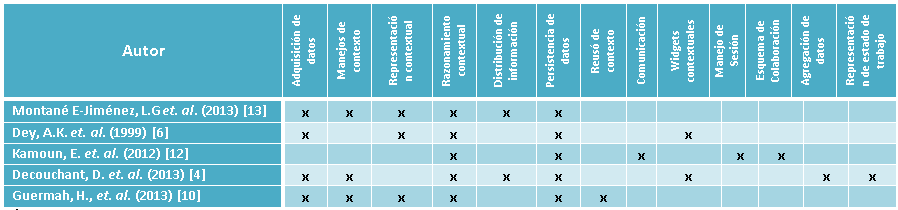
\includegraphics[scale=0.5]{images/comparaciones}
  \caption{Comparaci\'on de arquitecturas que soportan consciencia del contexto\cite{montane2013context}\cite{dey1999architecture}\cite{kamoun2012fadyrcos}\cite{decouchant2013adapting}\cite{guermah2013ontology}}
  \label{cmp:fig}
\end{figure}

\section{Modelo de Actividad}
En la literatura la mayor\'ia de modelos contextuales comparten elementos que comunmente describen cuatro factores t\'ipicos de contexto \cite{abowd1999towards}: ubicaci\'on, identidad, estado de las personas, grupos y objetos f\'isicos y virtuales. Algunos de estos modelos difieren en la forma de ser representados, o en el \'ambito en el que se aplican, desde representaci\'ones de espacios de trabajo \cite{decouchant2013adapting}, meta modelos que describen el comportamiento de un grupo de usuarios \cite{montane2013context} \cite{alves2013radiator} \cite{hoyos2013domain}, hasta aquellos modelos enfocados a las actividades de un usuario y su comportamiento \cite{kamoun2012fadyrcos}\cite{gallardo2012framework}\cite{guermah2013ontology}\cite{Doweling2012ATheory}. Para el presente trabajo se hace uso de un meta modelo contextual para el modelado de sistemas groupware basado un modelo propuesto anteriormente\cite{montane2013context}, en el cual se pueden encontrar dos categor\'ias de elementos, interactivos y cohesivos.  Entre los interactivos se encuentran \textit{actores}, que son los usuarios del sistema, \textit{objetos} que se usan en \textit{tareas} o que son producto de ellas, \textit{categor\'ias} que clasifican a los actores, objetos y tareas seg\'un sus atributos, por \'ultimo est\'an los roles del objeto y del actor los cuales son asignadas a una tarea para establecer el rol que va a tener el actor u objeto involucrado en dicha tarea. Entre los datos cohesivos se encuentran las \textit{comunidades} que son el conjunto de actores con una \textit{actividad} en com\'un, estas actividades pueden tener varias \textit{metas} las cuales se cumplen realizando tareas. Por \'ultimo se encuentran las reglas que son sentencias en un lenguaje definido para poder inferir las interacciones que suceden en el groupware. En la figura \ref{cmp:mmc} se muestra un diagrama de los elementos de este modelo y sus relaciones.

\begin{figure}[h!]
  \centering
    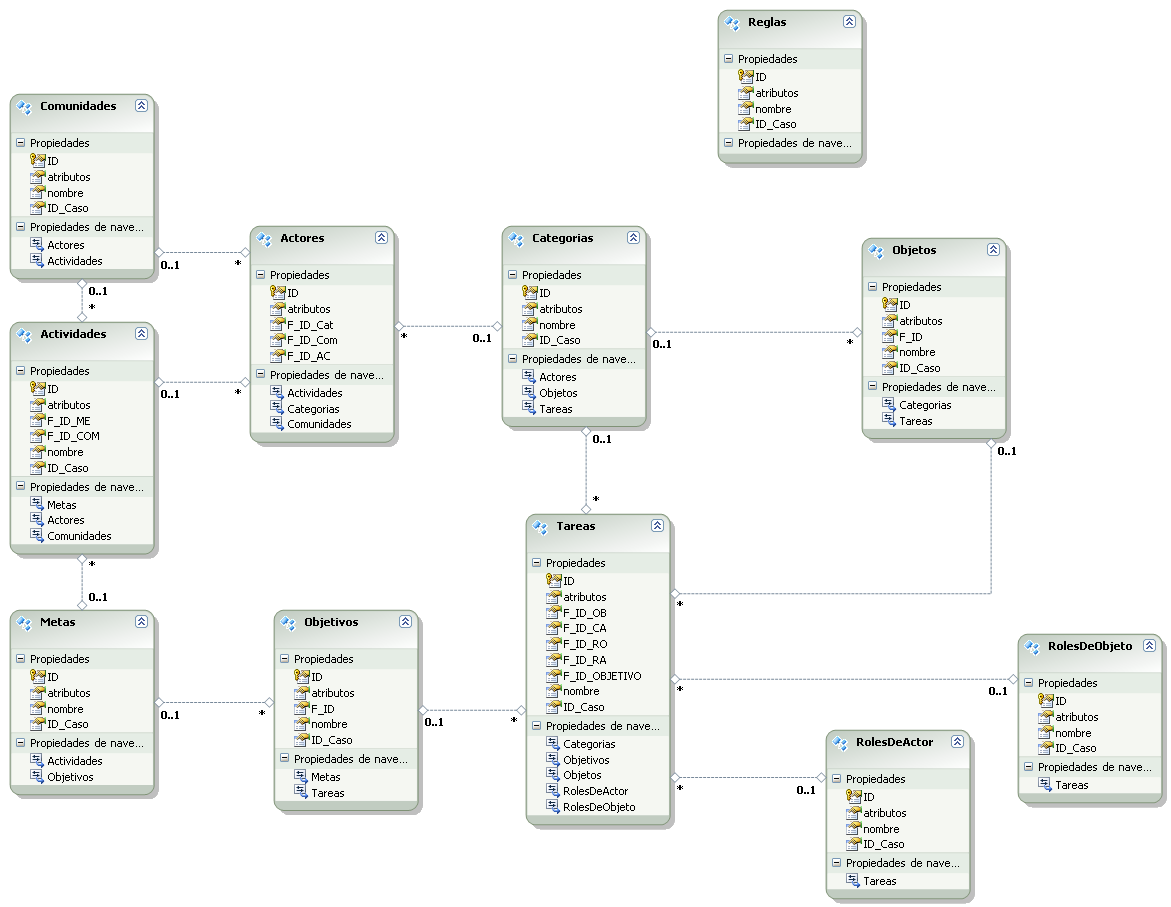
\includegraphics[scale=0.35]{images/modelo}
  \caption{Meta modelo contextual}
  \label{cmp:mmc}
\end{figure}

Con este meta modelo contextual se pueden describir groupwares definiendo cada uno de estos elementos a partir de interacciones, una vez dado de alta un caso junto con sus reglas se instancia un modelo que representar\'a al sistema colaborativo y almacenar\'a las variables contextuales que este transmita a la arquitectura. Cabe mencionar que en este metamodelo los elementos cuentan con 3 atributos principales, un identificador del objeto, un nombre descriptivo, y una lista de atributos almacenados en formato JSON, lo que vuelve flexible la forma de registrar casos de estudio.
\section{Caso de estudio}
Para el actual proyecto se necesita un groupware al cu\'al se le pueda acoplar la arquitectura para poder analizar sus datos, en este caso el sistema seleccionado es un videojuego colaborativo de disparos en primera persona: \textit{AssaultCube}. Este groupware en particular tiene las caracter\'isticas de ser distribuido y s\'incrono seg\'un la clasificaci\'on de Ellis\cite{ellis1991groupware}, contiene varios tipos de elementos y los modos multijugador son entre equipos en los cuales se requiere de una buena colaboraci\'on para cumplir los objetivos de la actividad. 

\begin{figure}[h!]
\centering
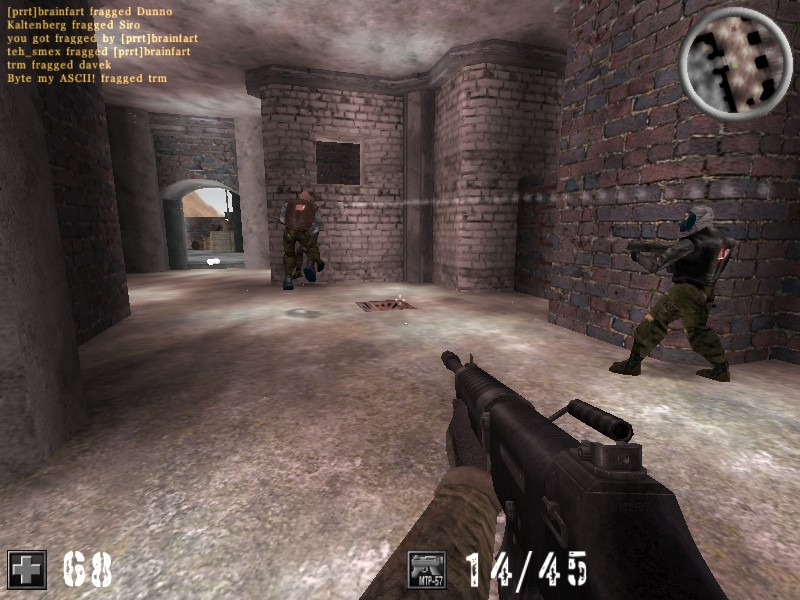
\includegraphics[scale=.15]{images/assaultcube}
\caption{Assault Cube}
\label{gw:asscb}
\end{figure}

En la Tabla 1 se muestran las interacciones identificadas en el juego, en ellas se encuentran algunos elementos del modelo como pueden ser Actores, Tareas y Objetos,  esto nos da la pauta para empeazar a dise\~nar nuestro modelo. 

\definecolor{LightCyan}{rgb}{0.29,0.67,0.77}
\begin{center}
\label{AC:interacciones}
\begin{longtable}{|p{5cm}|p{7cm}|}

\caption{Tabla de interacciones detectadas en \textit{Assault Cube}}\\
\hline
\rowcolor{LightCyan}\textbf{Interacci\'on} & \textbf{Elementos identificados}\\
\hline
\endfirsthead
\multicolumn{2}{c}%
{\tablename\ \thetable\ -- \textit{... Contin\'ua de p\'agina anterior}} \\
\hline
\textbf{Interacci\'on} & \textbf{Elementos identificados} \\
\hline
\endhead
\hline \multicolumn{2}{r}{\textit{Contin\'ua en siguiente p\'agina...}} \\
\endfoot
\hline
\endlastfoot
\textbf{Jugador se Mueve} & Actor: Jugador; Tarea: Moverse\\\hline

\textbf{Jugador salta} & Actor: Jugador; Tarea: Saltar\\\hline

\textbf{Jugador dispara arma} & Actor: Jugador; Tarea: Saltar; Objeto: Arma\\\hline

\textbf{Jugador recarga arma} & Actor: Jugador; Tarea: Recargar; Objeto: Arma\\\hline

\textbf{Jugador dispara arma} & Actor: Jugador; Tarea: Saltar; Objeto: Arma\\\hline

\textbf{Jugador cambia arma} & Actor: Jugador; Tarea: Cambiar; Objeto: Arma\\\hline

\textbf{Jugador obtiene mejora de salud} & Actor: Jugador; Tarea: Obtener; Objeto: Mejora de salud\\\hline

\textbf{Jugador obtiene protecci\'on} & Actor: Jugador; Tarea: Obtener; Objeto: Protecci\'on\\\hline

\textbf{Jugador obtiene munici\'on} & Actor: Jugador; Tarea: Obtener; Objeto: munici\'on\\\hline

\textbf{Jugador envia mensaje de texto} & Actor: Jugador; Tarea: enviar; Objeto: Mensaje de texto\\\hline

\textbf{Jugador envia mensaje de voz predefinido} & Actor: Jugador; Tarea: enviar; Objeto: Mensaje de voz\\\hline

\textbf{Jugador elige arma inicial} & Actor: Jugador; Tarea: Elegir; Objeto: Arma predeterminada\\\hline

\textbf{Jugador cambia rol} & Actor: Jugador; Tarea: Cambiar; Objeto: Rol\\\hline

\textbf{Jugador se agacha} & Actor: Jugador; Tarea: Agacharse\\\hline

\textbf{Jugador se suicida} & Actor: Jugador; Tarea: Suicidarse\\\hline

\textbf{Jugador es eliminado} & Actor: Jugador; Tarea: Ser eliminado\\\hline

\textbf{Jugador elimina oponente} & Actores: JugadorA, JugadorB; Tarea: Eliminar\\\hline

\textbf{Jugador reaparece} & Actor: Jugador; Tarea: Reaparecer\\\hline

\textbf{Jugador captura bandera} & Actor: Jugador; Tarea: Capturar; Objeto: Bandera\\\hline

\textbf{Jugador regresa bandera a su base} & Actor: Jugador; Tarea: Recuperar; Objeto: Bandera \\\hline

\textbf{Jugador ve mapa} & Actor: Jugador; Tarea: Ver; Objeto: Mapa\\\hline

\textbf{Jugador ve puntuaciones} & Actor: Jugador; Tarea: Ver; Puntuaciones\\\hline

\end{longtable}
\end{center}

En la lista anterior de interacciones se pueden identificar ya algunos elementos del modelo del groupware, por ejemplo, jugador como actor, arma, munici\'on, mapa como tipos de objetos, y el conjunto de ellos como tareas. Tambi\'en a partir de estas interacciones pueden empezar a definirse algunas reglas.


\section{Prototipo}
La arquitectura que se propone en este trabajo, como ya se mencion\'o antes cuenta con tres capas: recuperaci\'on de datos, gesti\'on de contexto, y uso de contexto. Para poder acoplar la arquitectura primero se tiene que dar de alta un modelo del groupware. Para esto se cre\'o una plataforma para registrar casos de estudio en la que se establece el nombre del caso de estudio y todos sus elementos, una vez creado el meta modelo del groupware se instancia el modelo de dominio del Groupware y se administran las interacciones para poder relacionar sus elementos, ya con este modelo se pueden capturar la informaci\'on contextual que el sistema va a enviar a la arquitectura. 

\begin{figure}[h!]
\centering
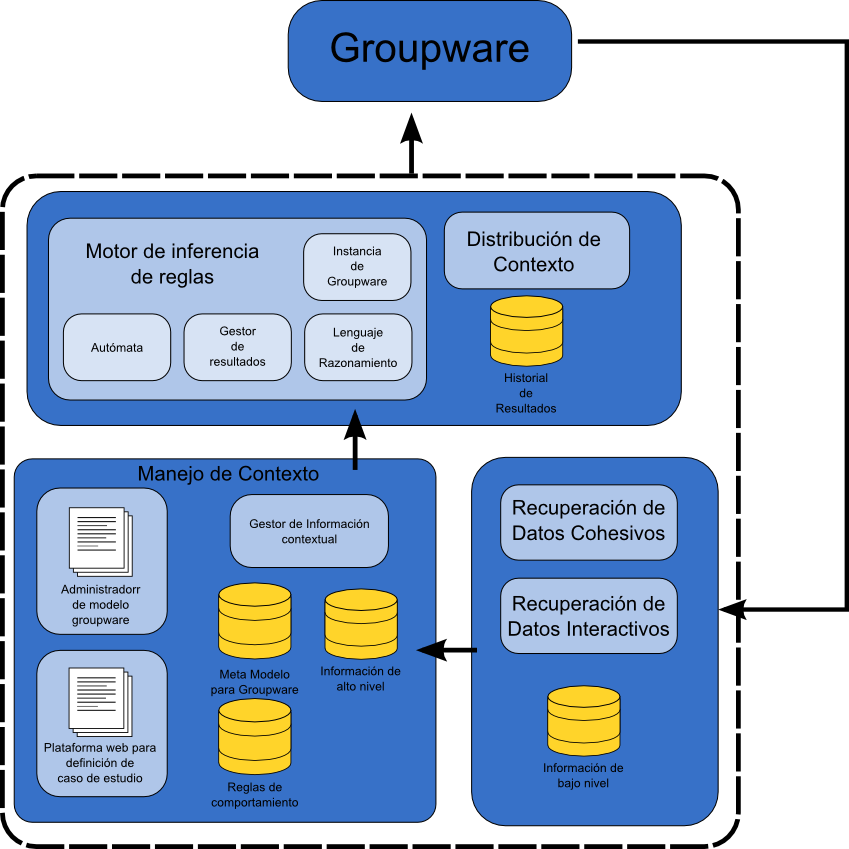
\includegraphics[scale=0.40]{images/arqui2}
\caption{Arquitectura propuesta}
\label{ARCH:propuesta}
\end{figure}

La arquitectura se divide en tres capas; la capa de recuperaci\'on de datos, la capa de gestion de datos y la capa de uso de contexto. En la primera capa, la de recuperac\'on de datos, se captura informaci\'on contextual enviada por el groupware por medio de servicios web din\'amicos, publicados para la comunicaci\'on entre la arquitectura y el sistema, estos datos son enviados en un formato espec\'ifico, en este caso serializados en Json. Seguido de este m\'odulo est\'a el de gesti\'on contextual, este gestor se encarga de registrar, actualizar y recuperar la informaci\'on contextual en bases de datos, es a este nivel donde se define el meta modelo y  se instancia el modelo de dominio del sistema y donde los datos enviados desde el groupware se registran, desde ahí son recuperados para inferir resultados en niveles superiores. Cabe mencionar que en esta plataforma tambi\'en se definen las reglas de comportamiento para el groupware. En estas reglas se definen los resultados que debe de arrojar el motor de inferencia basado en eventos del sistema, estos eventos se describen como interacciones, una interacci\'on $I$ esta compuesta b\'asicamente de un $Actor$ y una $Tarea$(\textit{e.g.} \textbf{Jugador se mueve}), a partir de este tipo de interaci\'on surgen otras, entre las que se identifican est\'an la interacci\'on en la que se afecta a otra entidad como un actor o conjunto de actores $A$ u objeto o conjunto de objetos $O$; y la interacci\'on en la que un actor $A$ realiza una tarea con ayuda de un objeto $O$. Adem\'as de las interacciones tambi\'en se da el caso en el que se necesiten comparar valores de los atributos de  los elementos, para esto se definieron las expresiones compuestas por un elemento del modelo de dominio, un atributo del elemento, un operador que compara el atributo con un valor v\'alido definido en el meta modelo, entre los operadores de comparaci\'on se encuentran '=', '\textless', '\textgreater', '$\neg$'(\textit{i.e.} de igualdad, mayor que, menor que, y diferencia).

En esta capa se encuentra una plataforma en la que se pueden dar de alta elementos del modelo de actividad. Para poder ingresar al sistema con un caso de estudio, se tiene que dar de alta con un nombre y una contrase\~na para el logueo, esto se lleva a cabo en la vista mostrada en la figura \ref{Ptf:registro1}

\begin{figure}
\centering
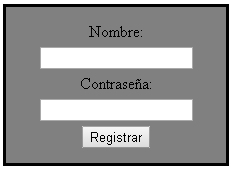
\includegraphics[scale=.8]{images/RegistroProto.png}
\caption{Registro de caso de estudio}
\label{Ptf:registro1}
\end{figure}

En la figura \ref{Ptf:login} se observa un formulario para le logueo al sistema, esto para poder asociar los elementos a un caso de estudio en espec\'ifico y los elementos est\'en disponibles s\'olo para los casos para los que fueron especificados.
\newpage
\begin{figure}[h!]
\centering
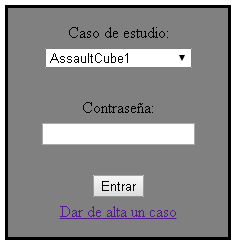
\includegraphics[scale=.7]{images/LoginProto.png}
\caption{Login de acceso a la plataforma.}
\label{Ptf:login}
\end{figure}

Una  vez dentro de la plataforma, en la pantalla principal mostrada en la figura\ref{Ptf:home} se encuentran pesta\~nas que dan acceso a las vistas de defnici\'on de los elementos del meta modelo y la pantalla para la definici\'on de reglas. Los elementos se encuentran divididos en elementos cohesivos e interactivos.

\begin{figure}[h!]
\centering
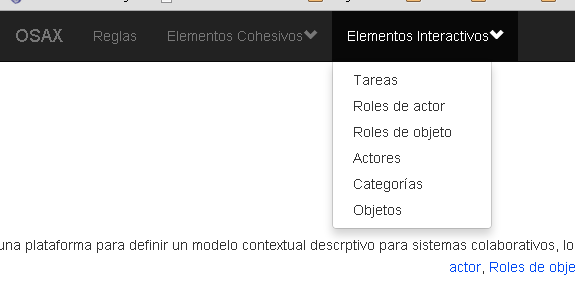
\includegraphics[scale=.7]{images/homeProto.png}
\caption{P\'agina inicial de la plataforma}
\label{Ptf:home}
\end{figure}

Al acceder a una vista de definici\'on de elemento, aparece un formulario similar a  la figura \ref{Ptf:registro} en la que se define el n\'umero de atributos, adicionales a los presentados, que van a formar parte del elemento del dominio del groupware y el valor que van a tomar, despu\'es de definir los atributos del elemento, se registra para que sea accesible por los elementos que puedan hacer uso de ellos.
\newpage

\begin{figure}[h!]
\centering
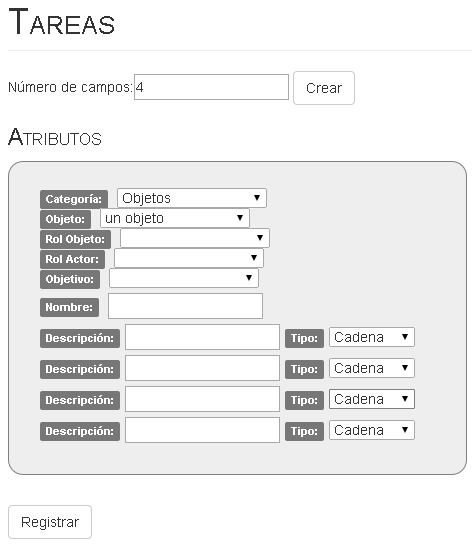
\includegraphics[scale=.6]{images/TareasProto.png}
\caption{Vista de registro de elementos}
\label{Ptf:registro}
\end{figure}

En la \'ultima capa de la arquitectura, uso de contexto, la informaci\'on es procesada por un motor de inferencia que trabaja con interacciones enviadas desde el groupware y  que da como resultado otra interacci\'on o conjunto de interacciones que representan una acci\'on propia del groupware que puede concluir en la presentaci\'on de informaci\'on al usuario que lo necesite o la ejecuci\'on de un comando para adaptar el groupware a la situaci\'on actual del usuario. Dentro del motor de inferencia se llevar\'a un registro de las instancias de las interacciones que se llevan a cabo en el groupware, as\'i se puede comparar su estado actual con las reglas de comportamiento definidas para ofrecer resultados coherentes en tiempo real. Los resultados obtenidos son gestionados por un administrador de resultados que almacena los datos para mantener registro hist\'orico del comportamiento del groupware. Una vez obtenidos y almacenados los resultados un m\'odulo de distribuci\'on se encarga de enviar las interacciones al groupware con la informaci\'on necesaria. Este proceso es iterativo, ya que funciona por el tiempo en el que el groupware opera.

\section{Conclusiones}
Esta arquitectura está diseñada para apoyar el trabajo colaborativo, pero su modelo se puede utlizar para brindar consciencia contexual a otro tipo de sistemas, se implementar\'a en el groupware Assault Cube y se probar\'an sus resultados, con esto se pretende evaluar el desempe\~no de la arquitectura. Har\'ia falta una interfaz acoplable al groupware para que este se pudiera comunicar con la arqutiectura con facilidad. La eficiencia de los resultados depende de las reglas definidas, si las reglas est\'an establecidas para apoyar al grupo de trabjo colaborativo entonces la arquitectura tambi\'en.
 
% use section* for acknowledgement
%\section*{Acknowledgment}
%Este trabajo es parte de un proyecto de investigación ``...'' por Conacyt y la Universidad Veracruzana.

% references section

\bibliographystyle{./bibtex/splncs03}
\bibliography{./bib/biblio}
\end{document}
